% -*-latex-*-
%\documentclass[pdftex,handout]{beamer}
\documentclass[pdftex,12pt]{beamer}
\usepackage{etex}
\let\latexput\put
\usepackage{pictex}
\let\pictexput\put
\let\put\latexput
\newcommand{\mutation}{$\cdot$}
\usepackage{ifthen}
\newcounter{showthis}
\setcounter{showthis}{1}
\newdimen\thusfar
\newdimen\plotht
\newdimen\plotwd
\newdimen\plotsp
\newdimen\xunit
\newdimen\yunit
\newdimen\offsety
\setbeamercovered{transparent}
\setbeamertemplate{footline}[frame number]
\author{Alan R. Rogers}
\date{\today}
\begin{document}

\title{Site Patterns and Population History: the Intuition that
  Underlies Legofit}
\frame{\titlepage}

\begin{frame}
  \frametitle{Notation for populations}
  \begin{columns}
    \column{0.3\textwidth}
    %-*-latex-*-
\let\put\pictexput
\mbox{\beginpicture
\headingtoplotskip=\baselineskip
\setcoordinatesystem units <0.35cm, 0.35cm>
\setplotarea x from 1 to 11, y from 1 to 13
\axis bottom invisible ticks length <0pt>
  withvalues {$X$} {$Y$} {$N$} /  at 2 6 10 / /
%\axis left ticks andacross numbered from 1 to 13 by 1 /
%\axis top ticks andacross numbered from 1 to 11 by 1 /
\setplotsymbol ({\normalsize .})
\plot 1 1 5 9 5 13 /
\plot 3 1 4 3 5 1 / 
\plot 7 1 5 5 6 7 8.75 1.5 /
\plot 10.75 1.5 7 9 7 13 /
\put {\textit{XY}} at 4 4
\put {\textit{XYN}} at 6 8
\endpicture}
\let\put\latexput

    \column{0.7\textwidth}
    \raggedleft
    $X$, $Y$, and $N$ are populations: African, European, and Neanderthal.

    \bigskip
    
    \textit{XY}: population ancestral to $X$ and $Y$.

    \bigskip
    
    \textit{XYN}: ancestral to $X$, $Y$, and $N$.
    \end{columns}
\end{frame}

\begin{frame}
  \frametitle{Nucleotide site patterns}
  \begin{columns}
    \column{0.3\textwidth}
    %-*-latex-*-
\let\put\pictexput
\mbox{\beginpicture
\headingtoplotskip=\baselineskip
\setcoordinatesystem units <0.35cm, 0.35cm>
\setplotarea x from 1 to 11, y from 1 to 13
\axis bottom invisible ticks length <0pt>
  withvalues {$X$} {$Y$} {$N$} /  at 2 6 10 / /
\axis bottom invisible shiftedto y=-0.3 ticks length <0pt>
withvalues {1} {1} {0} /  at 2 6 10 / /
%\axis left ticks andacross numbered from 1 to 13 by 1 /
%\axis top ticks andacross numbered from 1 to 11 by 1 /
\plotheading{Pattern \textit{xy}}
\setplotsymbol ({\normalsize .})
\plot 1 1 5 9 5 13 /
\plot 3 1 4 3 5 1 / 
\plot 7 1 5 5 6 7 8.75 1.5 /
\plot 10.75 1.5 7 9 7 13 /
\setplotsymbol ({\textcolor{gray}{\scriptsize .}})
\plot 2 1 4 5 4.5 6 /
\plot 6 1 4.5 3.5 4.5 5 4.5 6 /
\setplotsymbol ({\textcolor{red}{\scriptsize .}})
\plot 4.5 6 5 7 5.75 10 6 11 /
\setplotsymbol ({\textcolor{gray}{\scriptsize .}})
\plot 9.75 1.5 6.5 8 6 11 6 13 /
%\arrow <10pt> [.2,.67] from 8.5 2 to 6.5 2
\endpicture}
\let\put\latexput

    \column{0.7\textwidth}
    \raggedleft
    Haploid sample: 1 nucleotide from each population.

    \bigskip
    
    Mutation on red segment would appear in samples from $X$, $Y$, not
    that from $N$.

    \bigskip
    Call this the \textit{xy} site pattern.
  \end{columns}
  \bigskip\raggedleft I will write $xy\succ yn$ to mean that $xy$ is more
  common than $yn$.
\end{frame}

\begin{frame}
  \frametitle{Why haploid samples?}
  No variation within populations $\Rightarrow$ results not affected
  by recent history of population size.

  \bigskip

  The haploid samples are hypothetical; our real samples are
  larger. We use all the genomes in the real data to calculate the
  probability of observing site pattern \emph{xy} in a hypothetical
  haploid sample:
  \[
  \Pr[xy] = p_X p_Y (1-p_N)
  \]
  where $p_i$ is the frequency of the derived allele in the sample
  from population $i$. These site pattern frequencies are our data.
\end{frame}  

\begin{frame}
  \frametitle{Calling ancestral and derived alleles}
{\centering%auto-ignore
%-*-latex-*-
\let\put\pictexput
\mbox{\beginpicture
\headingtoplotskip=\baselineskip
\setcoordinatesystem units <0.5cm, 0.5cm> point at 7 0
\setplotarea x from 0 to 6, y from 0 to 7
\axis bottom invisible ticks length <0pt>
  withvalues {\llap{Allelic state:}} {C} {C} {T} {T} /  at -1 0 2 4 6 / /
%\axis left ticks andacross numbered from 1 to 7 by 1 /
%\axis top ticks andacross numbered from 1 to 6 by 1 /
\put {T} [b] <0pt,2pt> at 3 6
\put {$\bullet$} at 1.5 3
\plot 0 0 3 6 /
\plot 2 0 1 2 /
\plot 4 0 2 4 /
\plot 6 0 3 6 /
%%%%%%%%%%%%%%%%%%%%%%%%%%%%%%%%%%%%%%%%%%%%%%%%%%%%%%%%%%%%%%%%
\setcoordinatesystem units <0.5cm, 0.5cm> point at -1 0
\setplotarea x from 0 to 6, y from 0 to 7
\axis bottom invisible ticks length <0pt>
  withvalues {C} {C} {T} {T} /  at 0 2 4 6 / /
%\axis left ticks andacross numbered from 1 to 7 by 1 /
%\axis top ticks andacross numbered from 1 to 6 by 1 /
\put {C} [b] <0pt,2pt> at 3 6
\put {$\bullet$} at 3 2
\put {$\bullet$} at 5 2
\plot 0 0 3 6 /
\plot 2 0 1 2 /
\plot 4 0 2 4 /
\plot 6 0 3 6 /

\endpicture}
\let\put\latexput
\\}
    \bigskip
    
    2 mutations needed if $C$ is ancestral.

    \bigskip

    Only 1 needed if $T$ is ancestral.

    \bigskip

    Prefer hypothesis requiring fewer mutations, because mutations
    are rare.
\end{frame}

\begin{frame}
  \frametitle{Observed site pattern frequencies}
  \begin{columns}
    \column{0.7\textwidth}
    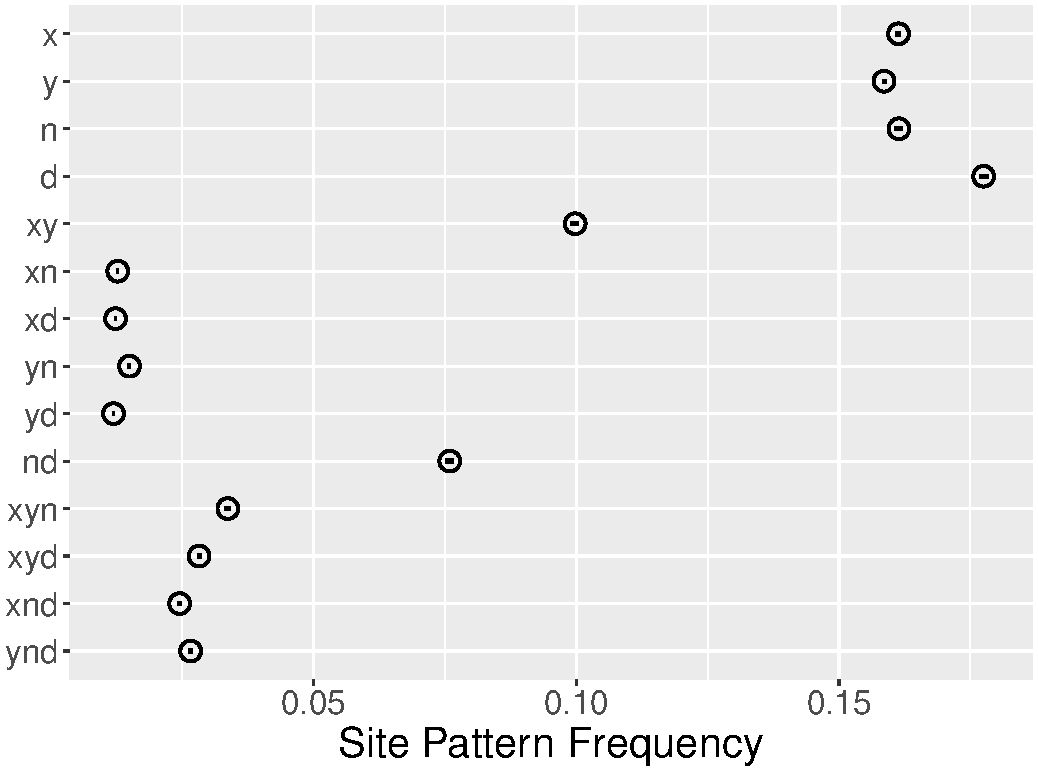
\includegraphics[width=\linewidth]{xynd-frq.pdf}
    \column{0.3\textwidth}
    \raggedleft

    $X$, Africa; $Y$, Europe; $N$, Neanderthal; $D$, Denisovan.

    \bigskip

    Horizontal axis: rel.\ freq.\ of each site pattern

    \bigskip

    ``Dots'' w/i circles are 95\% confidence intervals.
  \end{columns}
\end{frame}

\begin{frame}
  \frametitle{The pattern in the data}
  \begin{columns}
    \column{0.7\textwidth}
    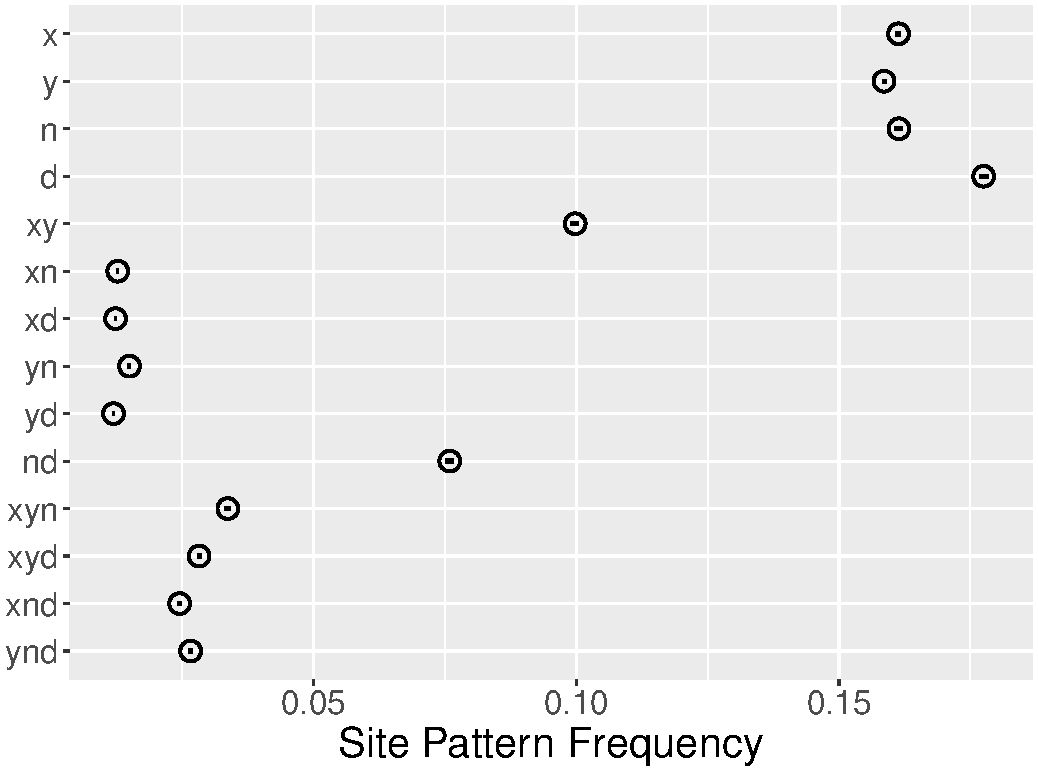
\includegraphics[width=\linewidth]{xynd-frq.pdf}
    \column{0.3\textwidth}
    \raggedleft

    Lots of singletons ($x$, $y$, $n$, and $d$)

    \bigskip

    Two doubletons (\textit{xy} and \textit{nd}) especially common

    \bigskip

    \textit{yn} more common than other rare doubletons.

    \bigskip

    \textit{xyn} more common than other tripletons.
  \end{columns}
  \bigskip\raggedleft
How can we understand this pattern?
\end{frame}

\begin{frame}
  \frametitle{1st pass: no frills}
  \begin{columns}
    \column{0.5\textwidth}
    %auto-ignore
%-*-latex-*-
\mbox{\beginpicture
\headingtoplotskip=\baselineskip
\setcoordinatesystem units <4mm, 3mm> point at 13 0
\setplotarea x from 0 to 13, y from 0 to 16
\axis bottom invisible ticks length <0pt>
  withvalues {$X$} {$Y$} {$N$} {$D$} /  at 1 5 8 12 / /
%\axis left ticks andacross numbered from 0 to 16 by 1 /
%\axis top ticks andacross numbered from 0 to 13 by 1 /
\plotheading{Early $N$-$D$ split} 
\setplotsymbol ({\normalsize .})
\plot 0 0 2 6 / %Xl
\plot 2 6 5.5 13 / % XYl
\plot 2 0 3 3 / %Xr
\plot 4 0 3 3 / %Yl
\plot 6 0 4 5 / %Yr
\plot 4 5 6.5 10.5 / %XYr
\plot 7 0 8 6 9 8 / %Nl
\plot 9 0 10 6 / %Nr
\plot 11 0 10 6 / %Dl
\plot 13 0 12 6 10.5 10 / %Dr
\plot 9 8 6.5 10.5 / %NDl
\plot 10.5 10 7.5 13 / %NDr
\plot 5.5 13 5.5 16 / %XYNDl
\plot 7.5 13 7.5 16 / %XYNDr
\setplotsymbol ({\textcolor{gray}{\scriptsize .}})
\plot 1 0 2.5 5 3.33 6 / %x
\plot 5 0 3.5 4 3.33 6 / %y
\setplotsymbol ({\textcolor{blue}{\scriptsize .}})
\plot 3.33 6 6 12 6.5 15 / %xy
\setplotsymbol ({\textcolor{gray}{\scriptsize .}})
\plot 8 0 9 6 9.4 8.4 9 9.75 / %n
\plot 12 0 11 6 10 9.3 9 9.75 / %d
\setplotsymbol ({\textcolor{red}{\scriptsize .}})
\plot 9 9.75 7 11.75 6.5 15 / %nd
\setplotsymbol ({\textcolor{gray}{\scriptsize .}})
\plot 6.5 15 6.5 16 / %xynd
\endpicture}

    \column{0.5\textwidth}
    \raggedleft
    No gene flow; gene genealogy matches population tree.

    \bigskip

    Many other genealogies are possible, but this one will be common.

    \bigskip

    Captures large-scale pattern; misses subtleties.
  \end{columns}
\end{frame}

\begin{frame}
  \frametitle{Why are \textit{xy} and \textit{nd} so common?}
  \begin{columns}
    \column{0.5\textwidth}
    %auto-ignore
%-*-latex-*-
\mbox{\beginpicture
\headingtoplotskip=\baselineskip
\setcoordinatesystem units <4mm, 3mm> point at 13 0
\setplotarea x from 0 to 13, y from 0 to 16
\axis bottom invisible ticks length <0pt>
  withvalues {$X$} {$Y$} {$N$} {$D$} /  at 1 5 8 12 / /
%\axis left ticks andacross numbered from 0 to 16 by 1 /
%\axis top ticks andacross numbered from 0 to 13 by 1 /
\plotheading{Early $N$-$D$ split} 
\setplotsymbol ({\normalsize .})
\plot 0 0 2 6 / %Xl
\plot 2 6 5.5 13 / % XYl
\plot 2 0 3 3 / %Xr
\plot 4 0 3 3 / %Yl
\plot 6 0 4 5 / %Yr
\plot 4 5 6.5 10.5 / %XYr
\plot 7 0 8 6 9 8 / %Nl
\plot 9 0 10 6 / %Nr
\plot 11 0 10 6 / %Dl
\plot 13 0 12 6 10.5 10 / %Dr
\plot 9 8 6.5 10.5 / %NDl
\plot 10.5 10 7.5 13 / %NDr
\plot 5.5 13 5.5 16 / %XYNDl
\plot 7.5 13 7.5 16 / %XYNDr
\setplotsymbol ({\textcolor{gray}{\scriptsize .}})
\plot 1 0 2.5 5 3.33 6 / %x
\plot 5 0 3.5 4 3.33 6 / %y
\setplotsymbol ({\textcolor{blue}{\scriptsize .}})
\plot 3.33 6 6 12 6.5 15 / %xy
\setplotsymbol ({\textcolor{gray}{\scriptsize .}})
\plot 8 0 9 6 9.4 8.4 9 9.75 / %n
\plot 12 0 11 6 10 9.3 9 9.75 / %d
\setplotsymbol ({\textcolor{red}{\scriptsize .}})
\plot 9 9.75 7 11.75 6.5 15 / %nd
\setplotsymbol ({\textcolor{gray}{\scriptsize .}})
\plot 6.5 15 6.5 16 / %xynd
\endpicture}

    \column{0.5\textwidth}
    \raggedleft
    Mutation on blue $\rightarrow$ \textit{xy};
    mutation on red $\rightarrow$ \textit{nd}.

    \bigskip

    \textit{xy} and \textit{nd} are common because $X$ and $Y$ are
    closely related, as are $N$ and $D$.
  \end{columns}
\end{frame}

\begin{frame}
  \frametitle{Why is $xy \succ nd$?}
  \begin{columns}
    \column{0.5\textwidth}
    %auto-ignore
%-*-latex-*-
\mbox{\beginpicture
\headingtoplotskip=\baselineskip
\setcoordinatesystem units <4mm, 3mm> point at 13 0
\setplotarea x from 0 to 13, y from 0 to 16
\axis bottom invisible ticks length <0pt>
  withvalues {$X$} {$Y$} {$N$} {$D$} /  at 1 5 8 12 / /
%\axis left ticks andacross numbered from 0 to 16 by 1 /
%\axis top ticks andacross numbered from 0 to 13 by 1 /
\plotheading{Early $N$-$D$ split} 
\setplotsymbol ({\normalsize .})
\plot 0 0 2 6 / %Xl
\plot 2 6 5.5 13 / % XYl
\plot 2 0 3 3 / %Xr
\plot 4 0 3 3 / %Yl
\plot 6 0 4 5 / %Yr
\plot 4 5 6.5 10.5 / %XYr
\plot 7 0 8 6 9 8 / %Nl
\plot 9 0 10 6 / %Nr
\plot 11 0 10 6 / %Dl
\plot 13 0 12 6 10.5 10 / %Dr
\plot 9 8 6.5 10.5 / %NDl
\plot 10.5 10 7.5 13 / %NDr
\plot 5.5 13 5.5 16 / %XYNDl
\plot 7.5 13 7.5 16 / %XYNDr
\setplotsymbol ({\textcolor{gray}{\scriptsize .}})
\plot 1 0 2.5 5 3.33 6 / %x
\plot 5 0 3.5 4 3.33 6 / %y
\setplotsymbol ({\textcolor{blue}{\scriptsize .}})
\plot 3.33 6 6 12 6.5 15 / %xy
\setplotsymbol ({\textcolor{gray}{\scriptsize .}})
\plot 8 0 9 6 9.4 8.4 9 9.75 / %n
\plot 12 0 11 6 10 9.3 9 9.75 / %d
\setplotsymbol ({\textcolor{red}{\scriptsize .}})
\plot 9 9.75 7 11.75 6.5 15 / %nd
\setplotsymbol ({\textcolor{gray}{\scriptsize .}})
\plot 6.5 15 6.5 16 / %xynd
\endpicture}

    \column{0.5\textwidth}
    \raggedleft
    Blue branch is longer than red, because $X$ and $Y$ separated more
    recently than $N$ and $D$.

    \bigskip

    Explains why $xy \succ nd$.
  \end{columns}
\end{frame}

\begin{frame}
  \frametitle{Data again: \textit{xy} and \textit{nd} common, but
  $xy \succ nd$}
    {\centering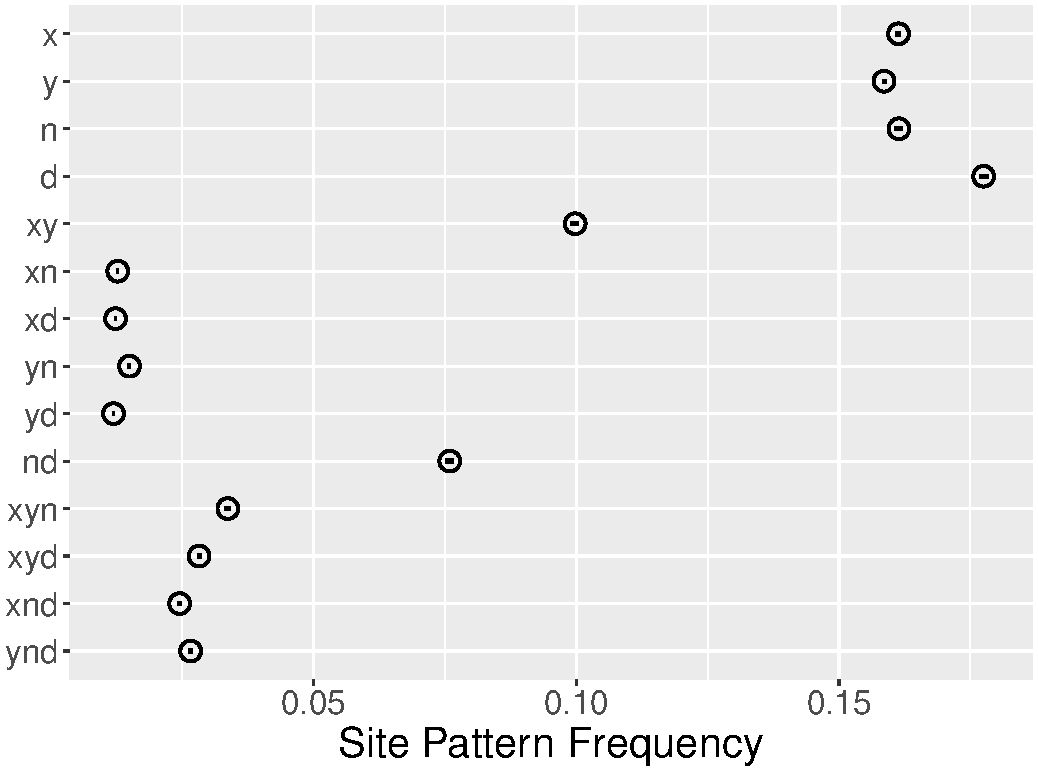
\includegraphics[width=0.9\linewidth]{xynd-frq.pdf}\\}
\end{frame}

\begin{frame}
  \frametitle{An alternate hypothesis}
  \begin{columns}
    \column{0.5\textwidth}
    %auto-ignore
%-*-latex-*-
\mbox{\beginpicture
\headingtoplotskip=\baselineskip
\setcoordinatesystem units <4mm, 3mm> point at -1 0
\setplotarea x from 0 to 13, y from 0 to 16
\axis bottom invisible ticks length <0pt>
  withvalues {$X$} {$Y$} {$N$} {$D$} /  at 1 5 8 12 / /
%\axis left ticks andacross numbered from 0 to 16 by 1 /
%\axis top ticks andacross numbered from 0 to 13 by 1 /
\plotheading{Large \textit{ND}} 
\setplotsymbol ({\normalsize .})
\plot 0 0 2 6 / %Xl
\plot 2 6 5.5 13 / % XYl
\plot 2 0 3 3 / %Xr
\plot 4 0 3 3 / %Yl
\plot 6 0 4 5 / %Yr
\plot 4 5 6 9 / %XYr
\plot 7 0 8.5 4 / %Nl
\plot 9 0 10 3 / %Nr
\plot 11 0 10 3 / %Dl
\plot 13 0 11 6 / %Dr
\plot 8.5 4 6 9 / %NDl
\plot 11 6 7.5 13 / %NDr
\plot 5.5 13 5.5 16 / %XYNDl
\plot 7.5 13 7.5 16 / %XYNDr
\setplotsymbol ({\textcolor{gray}{\scriptsize .}})
\plot 1 0 2.5 5 3.33 6 / %x
\plot 5 0 3.5 4 3.33 6 / %y
\setplotsymbol ({\textcolor{blue}{\scriptsize .}})
\plot 3.33 6 6 12 6.5 15 / %xy
\setplotsymbol ({\textcolor{gray}{\scriptsize .}})
\plot 8 0 9.5 4 7 10.5 / %n
\plot 12 0 10.5 5 7 10.5 / %d
\setplotsymbol ({\textcolor{red}{\scriptsize .}})
\plot 7 10.5 6.5 15 / %nd
\setplotsymbol ({\textcolor{gray}{\scriptsize .}})
\plot 6.5 15 6.5 16 / %xynd
\endpicture}

    \column{0.5\textwidth}
    \raggedleft
    Separation times are equal.

    \bigskip
    
    But $ND$ is large, so coalescence is slow, and red branch is short.

    \bigskip

    $xy \succ nd$ because $ND$ is larger than $XY$.

    \bigskip

    The two hypotheses are hard to tell apart.
  \end{columns}
\end{frame}

\begin{frame}
  \frametitle{Counterintuitive site patterns}
  {\centering%-*-latex-*-
\let\put\pictexput
\mbox{\beginpicture
\headingtoplotskip=\baselineskip
\setcoordinatesystem units <0.4cm, 0.4cm> point at 12 1
\setplotarea x from 1 to 11, y from 1 to 13
\axis bottom invisible ticks length <0pt>
  withvalues {$X$} {$Y$} {$N$} /  at 2 6 10 / /
\axis bottom invisible shiftedto y=-0.3 ticks length <0pt>
  withvalues {1} {0} {1} / at 2 6 10 / /
%\axis left ticks andacross numbered from 1 to 13 by 1 /
%\axis top ticks andacross numbered from 1 to 11 by 1 /
\plotheading{Pattern \textit{xn}}
\setplotsymbol ({\normalsize .})
\plot 1 1 5 9 5 13 /
\plot 3 1 4 3 5 1 / 
\plot 7 1 5 5 6 7 9 1 /
\plot 11 1 7 9 7 13 /
\setplotsymbol ({\textcolor{gray}{\scriptsize .}})
\plot 2 1  6 9 /
\plot 6 12 6 13 / % xyn
\plot 6 1 4.5 3.5 4.5 5 6.5 9 6 12 / %y
\setplotsymbol ({\textcolor{red}{\scriptsize .}})
\plot 6 9  6 12 / % x
\setplotsymbol ({\textcolor{gray}{\scriptsize .}})
\plot 10 1 6 9 / %n
%\arrow <10pt> [.2,.67] from 8.5 2 to 6.5 2
%%%%%%%%%%%%%%%%%%%%%%%%%%%%%%%%%%%%%%%%%%%%%%%%%%%%%%%%%%%%%%%%
\setcoordinatesystem units <0.4cm, 0.4cm> point at 0 1
\setplotarea x from 1 to 11, y from 1 to 13
\axis bottom invisible ticks length <0pt>
  withvalues {$X$} {$Y$} {$N$} /  at 2 6 10 / /
\axis bottom invisible shiftedto y=-0.3 ticks length <0pt>
  withvalues {0} {1} {1} / at 2 6 10 / /
%\axis left ticks andacross numbered from 1 to 13 by 1 /
%\axis top ticks andacross numbered from 1 to 11 by 1 /
\plotheading{Pattern \textit{yn}}
\setplotsymbol ({\normalsize .})
\plot 1 1 5 9 5 13 /
\plot 3 1 4 3 5 1 / 
\plot 7 1 5 5 6 7 9 1 /
\plot 11 1 7 9 7 13 /
\setplotsymbol ({\textcolor{gray}{\scriptsize .}})
\plot 2 1  6 9 6 13 /
\plot 6 1 4.5 3.5 4.5 5 6.5 9 / %y
\setplotsymbol ({\textcolor{red}{\scriptsize .}})
\plot 6.5 9  6 12 / % x
\setplotsymbol ({\scriptsize .})
\plot 10 1 6.5 8 6.5 9 / %n
%\arrow <10pt> [.2,.67] from 8.5 2 to 6.5 2
\endpicture}
\let\put\latexput
\\}  
\end{frame}

\begin{frame}
  \frametitle{Incomplete lineage sorting}
  Suppose that, as we trace the ancestry of our sample backwards in
  time, the lineages from $X$ and $Y$ don't
  coalesce until we reach \textit{XYN}.

  \bigskip

  Then there are three lineages, $X$, $Y$, and $N$, in the same
  population.

  \bigskip

  They can coalesce in any order.

  \bigskip

  Site patterns \textit{xy}, \textit{xn}, and \textit{yn} are equally
  likely.

  \bigskip

  This process is called ``incomplete lineage sorting.''
\end{frame}  

\begin{frame}
  \frametitle{Pattern \textit{xy} can also arise another way}
  \begin{columns}
    \column{0.3\textwidth}
    %-*-latex-*-
\let\put\pictexput
\mbox{\beginpicture
\headingtoplotskip=\baselineskip
\setcoordinatesystem units <0.35cm, 0.35cm>
\setplotarea x from 1 to 11, y from 1 to 13
\axis bottom invisible ticks length <0pt>
  withvalues {$X$} {$Y$} {$N$} /  at 2 6 10 / /
\axis bottom invisible shiftedto y=-0.3 ticks length <0pt>
withvalues {1} {1} {0} /  at 2 6 10 / /
%\axis left ticks andacross numbered from 1 to 13 by 1 /
%\axis top ticks andacross numbered from 1 to 11 by 1 /
\plotheading{Pattern \textit{xy}}
\setplotsymbol ({\normalsize .})
\plot 1 1 5 9 5 13 /
\plot 3 1 4 3 5 1 / 
\plot 7 1 5 5 6 7 8.75 1.5 /
\plot 10.75 1.5 7 9 7 13 /
\setplotsymbol ({\textcolor{gray}{\scriptsize .}})
\plot 2 1 4 5 4.5 6 /
\plot 6 1 4.5 3.5 4.5 5 4.5 6 /
\setplotsymbol ({\textcolor{red}{\scriptsize .}})
\plot 4.5 6 5 7 5.75 10 6 11 /
\setplotsymbol ({\textcolor{gray}{\scriptsize .}})
\plot 9.75 1.5 6.5 8 6 11 6 13 /
%\arrow <10pt> [.2,.67] from 8.5 2 to 6.5 2
\endpicture}
\let\put\latexput

    \column{0.7\textwidth}
    \raggedleft
    The lineages from $X$ and $Y$ may also coalesce w/i \textit{XY},
    generating site pattern \textit{xy}.

    \bigskip
    
    So $xy \succ xn, yn$.

    \bigskip

    \textit{xn} and \textit{yn} should be equally common.
  \end{columns}

  \bigskip\raggedleft
  
This is the pattern expected in the absence of gene flow.
\end{frame}

\begin{frame}
  \frametitle{Does incomplete lineage sorting (ILS) explain the data?}
  \begin{columns}
    \column{0.7\textwidth}
    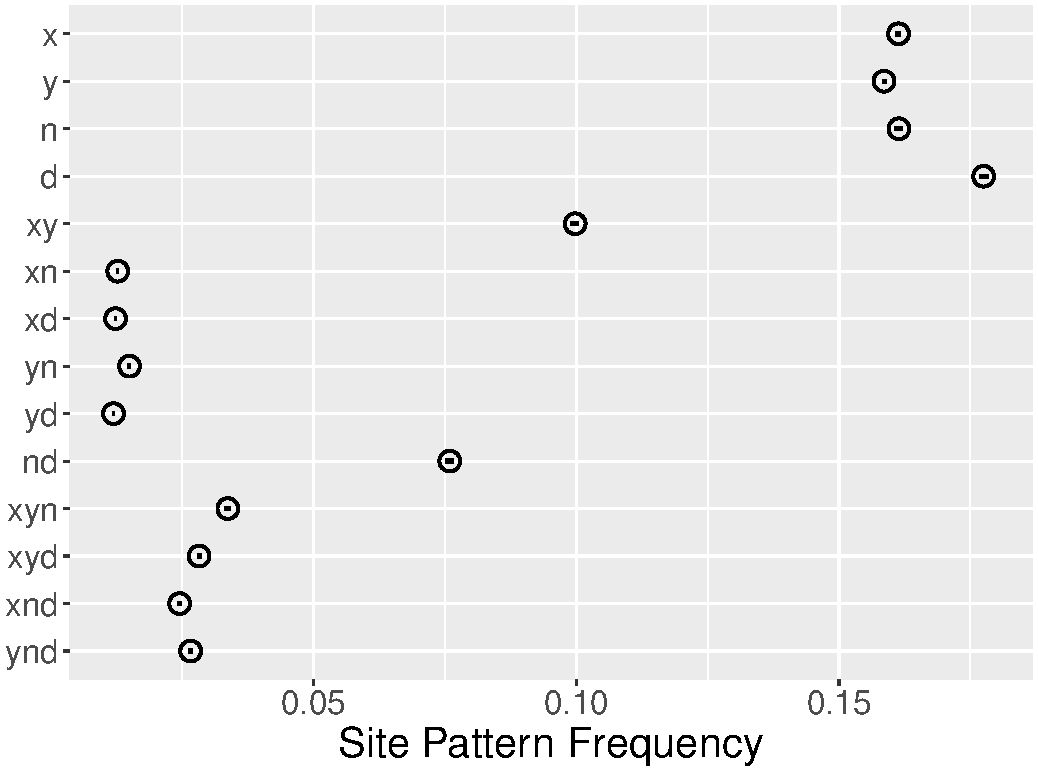
\includegraphics[width=\linewidth]{xynd-frq.pdf}
    \column{0.3\textwidth}
    \raggedleft

    \textit{xd} and \textit{yd} have equal frequencies, as they should
    under ILS.

    \bigskip

    But $yn \succ xn$, and the difference $>$ the confidence intervals.

    \bigskip

    Why?

  \end{columns}
  \bigskip\raggedleft
\end{frame}

\begin{frame}
  \frametitle{The effect of gene flow}
  \begin{columns}
  \column{0.7\textwidth}
  %-*-latex-*-
\let\put\pictexput
\mbox{\beginpicture
\headingtoplotskip=\baselineskip
\setcoordinatesystem units <0.35cm, 0.35cm> point at 12 1
\setplotarea x from 1 to 11, y from 1 to 13
\axis bottom invisible ticks length <0pt>
  withvalues {$X$} {$Y$} {$N$} /  at 2 6 10 / /
\axis bottom invisible shiftedto y=-0.3 ticks length <0pt>
withvalues  {1} {0} {0} /  at 2 6 10 / /
%\axis left ticks andacross numbered from 1 to 13 by 1 /
%\axis top ticks andacross numbered from 1 to 11 by 1 /
\plotheading{Without admixture}
\setplotsymbol ({\normalsize .})
\plot 1 1 5 9 5 13 /
\plot 3 1 4 3 5 1 / 
\plot 7 1 5 5 6 7 9 1 /
\plot 11 1 7 9 7 13 /
\setplotsymbol ({\textcolor{gray}{\scriptsize .}})
\plot 4 5 5 7 5.75 10 6 11 6 13 / %x
\plot 6 1 4 5 / %y
\setplotsymbol ({\textcolor{blue}{\scriptsize .}})
\plot 2 1 4 5  / %x
\setplotsymbol ({\textcolor{gray}{\scriptsize .}})
\plot 8.5 4 6.5 8 6 11 / %n
\setplotsymbol ({\textcolor{gray}{\scriptsize .}})
\plot 10 1 8.5 4 / %n
\setplotsymbol ({\normalsize .})
%\arrow <10pt> [.2,.67] from 8.5 2 to 6.5 2
%%%%%%%%%%%%%%%%%%%%%%%%%%%%%%%%%%%%%%%%%%%%%%%%%%%%%%%%%%%%%%%%
\setcoordinatesystem units <0.35cm, 0.35cm> point at -1 1
\setplotarea x from 1 to 11, y from 1 to 13
\axis bottom invisible ticks length <0pt>
  withvalues {$X$} {$Y$} {$N$} /  at 2 6 10 / /
\axis bottom invisible shiftedto y=-0.3 ticks length <0pt>
withvalues {1} {0} {0} /  at 2 6 10 / /
\axis bottom invisible shiftedto y=-1.3 ticks length <0pt>
withvalues  {0} {1} {1} /  at 2 6 10 / /
%\axis left ticks andacross numbered from 1 to 13 by 1 /
%\axis top ticks andacross numbered from 1 to 11 by 1 /
\plotheading{With admixture}
\setplotsymbol ({\normalsize .})
\plot 1 1 5 9 5 13 /
\plot 3 1 4 3 5 1 / 
\plot 7 1 5 5 6 7 9 1 /
\plot 11 1 7 9 7 13 /
\setplotsymbol ({\textcolor{gray}{\scriptsize .}})
\plot 2 1 5 7 5.75 10 6 11 6 13 / %x
\plot 6 1 5.5 2 9 2  8.5 4 / %y
\setplotsymbol ({\textcolor{blue}{\scriptsize .}})
\plot 2 1 5 7 5.75 10 6 11 / %x
\setplotsymbol ({\textcolor{red}{\scriptsize .}})
\plot 8.5 4 6.5 8 6 11 /
\setplotsymbol ({\textcolor{gray}{\scriptsize .}})
\plot 10.5 1 8.5 4 / %n
\setplotsymbol ({\normalsize .})
\arrow <10pt> [.2,.67] from 8.5 2 to 6.5 2
\endpicture}
\let\put\latexput

  \column{0.3\textwidth}
  \raggedleft

  $N{\rightarrow}Y$ gene flow inflates the frequency of \textit{yn}.

  \bigskip

  Also inflates frequency of $x$.

  \bigskip

  Effects are small unless the rate of gene flow is high.
  \end{columns}
\end{frame}


\begin{frame}
  \frametitle{Data are consistent with $N{\rightarrow}Y$ gene flow}
  \begin{columns}
    \column{0.7\textwidth}
    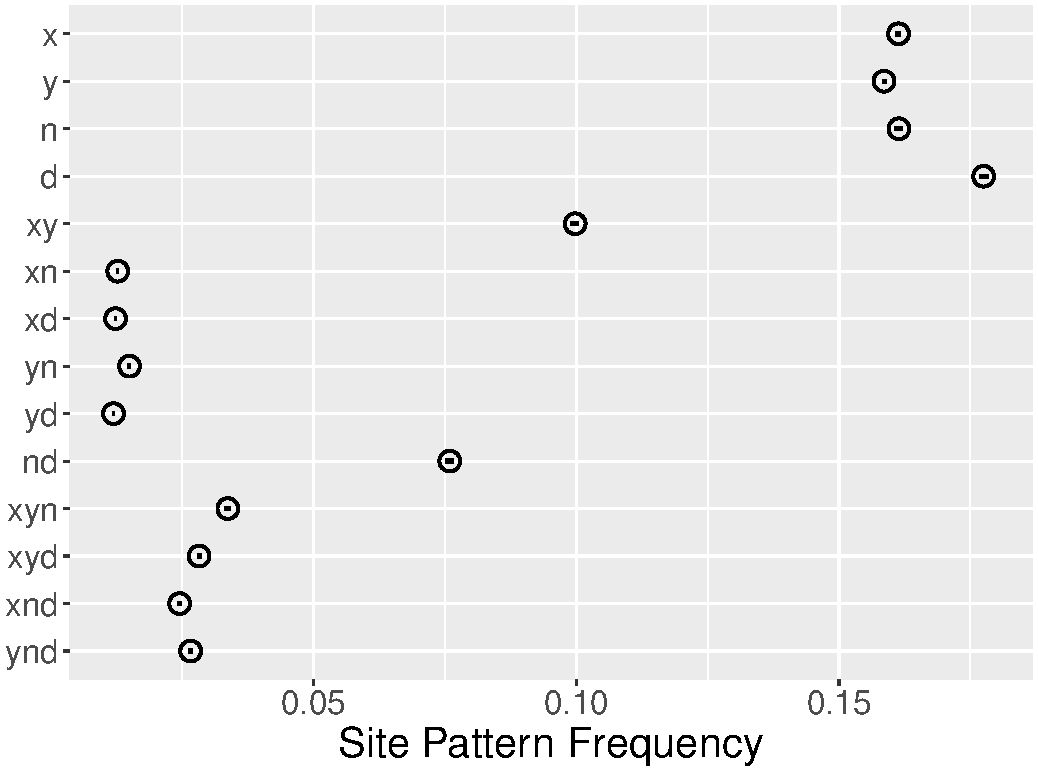
\includegraphics[width=\linewidth]{xynd-frq.pdf}
    \column{0.3\textwidth}
    \raggedleft

    $yn \succ xn$, and $x \succ y$.

    \bigskip

    Signature of $N{\rightarrow}Y$ gene flow.
    
  \end{columns}
\end{frame}

\begin{frame}
  \frametitle{Puzzling excess of $d$ site pattern}
  \begin{columns}
    \column{0.7\textwidth}
    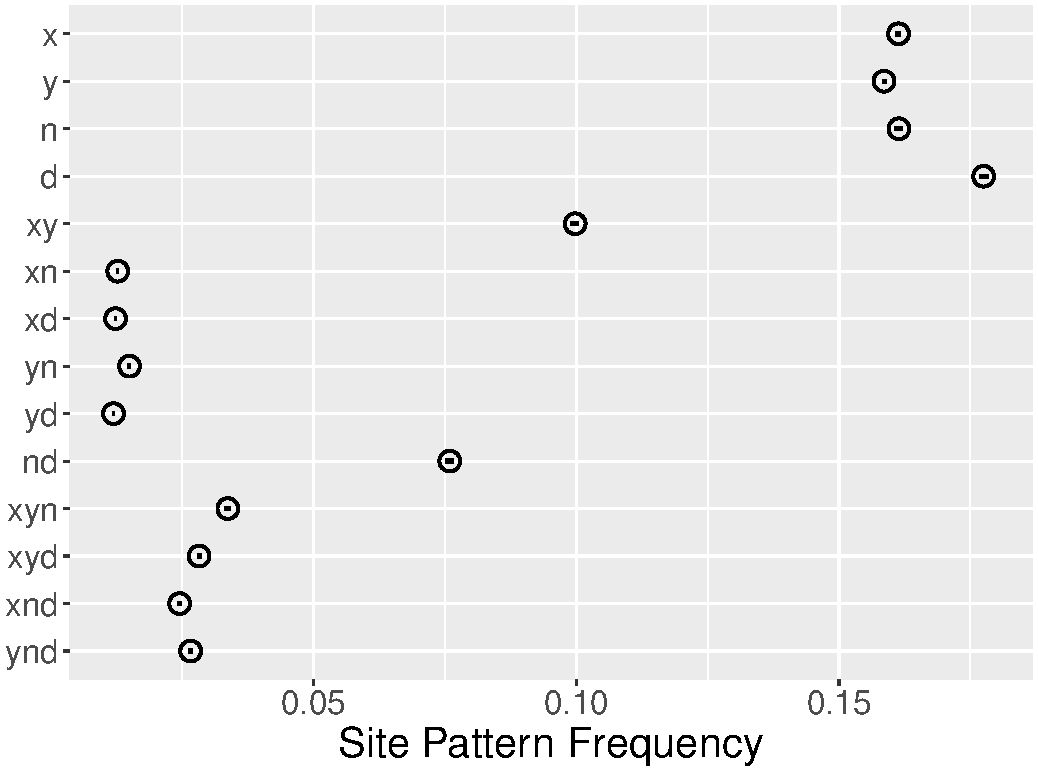
\includegraphics[width=\linewidth]{xynd-frq.pdf}
    \column{0.3\textwidth}
      \raggedleft

      $d$ is most common singleton

      \bigskip

      Suggests Denisovan fossil is young and $N$-$D$ separation old.

      \bigskip

      But our 2017 analysis of this hypothesis led to absurd result:
      Denisovan fossil only 4000 y old.
  \end{columns}

  \bigskip\raggedleft
      
  Something was missing from our model
\end{frame}

\begin{frame}
  \frametitle{Admixture from superarchaics into Denisovans}
  \begin{columns}
    \column{0.7\textwidth}
    %auto-ignore
%-*-latex-*-
\let\put\pictexput
\mbox{\beginpicture
\headingtoplotskip=\baselineskip
\setcoordinatesystem units <3.4mm, 3mm>
\setplotarea x from -2 to 17.5, y from 0 to 20
\axis bottom invisible ticks length <0pt>
  withvalues {$X$} {$Y$} {$N$} {$D$} {$S$} /  at 1 6 9 13 17 / /
\color{red}
\axis bottom invisible shiftedto y=-1.3 ticks length <0pt>
  withvalues {\llap{$d$:}} {0} {0} {0} {1} /
  at 0 1 6 9 13 / /
\color{blue}
\axis bottom invisible shiftedto y=-2.6 ticks length <0pt>
  withvalues {\llap{$xyn$:}} {1} {1} {1} {0} /
  at 0 1 6 9 13 / /
\color{black} % I issue this command twice, because otherwise,
\color{black} % the rest of the document is blue.
%\axis left ticks andacross numbered from 0 to 20 by 2 /
%\axis top ticks andacross numbered from 0 to 20 by 2 /
\setplotsymbol ({\normalsize .})
\plot 0 0 6 12 6 20 /   %X
\plot 2 0 3.5 3 5 0 /   %XY
\plot 7 0 4.5 5 7.12486206354179 10.249724127083585 /    %Y
%\arrow <10pt> [.2, .67] from 13.7 9 to 10.6 9
%\put {\small $\delta$} [t]  <0pt,-5pt> at 12.9 9
%\put {\small $\gamma$} [b]  <0pt,5pt> at 7.3 6
%\arrow <10pt> [.2,.67] from 5 6 to 9.6 6
\plot 8.17572 0 9.1757 5 10.036 6.7206 / %N
\plot 10 0 11 5 /       %N
\plot 12 0 11 5 /            %D
\plot 8 16 14.21226360816738 8.468963009740001 15.684 0 / %Sl
\plot 8 20 8 18.8112 15.8936 9.24189 17.4997 0 / %Sr
\plot 13.684 0 12.8151 5 11.3389 7.9523 8 12 8 16 / %Dr
\plot 7.12486206354179 10.249724127083585 10.036 6.7206 / % ND l
\arrow <10pt> [.2,.67] from 8.57571931984138 2 to 6 2
%\arrow <0pt> [.2,.67] from 11.75 1 to 10.25 1
%\arrow <10pt> [.2,.67] from 8.32572 1 to 6.5 1
\put {\small $\alpha$} [b]  <0pt,5pt> at 7.5 2
%\put {\small $\epsilon$} [t]  <0pt,-5pt> at 11 1
\put {\small $\beta$} [b]  <0pt,5pt> at 13.9889 4
\arrow <10pt> [.2,.67] from 14.9889 4 to 12.9889 4
\setplotsymbol ({\textcolor{gray}{\scriptsize .}})
\plot 1 0 7 12 7 13 /         % x, xy, bottom of xynd
\setplotsymbol ({\textcolor{blue}{\scriptsize .}})
\plot 7 13 7 20 /             % top of xynd
\setplotsymbol ({\textcolor{gray}{\scriptsize .}})
%\plot 6 0 5 2 9 2 9.8879 4 /  %y
\plot 6 0 4 4 4 6 / %y
\plot
   12.649562539059012 0.5
   11.946500312472102 4
   12.9889 4
/ % d
\plot
   9.187899999999999 0.5
   9.8879 4
   10.581012916966557 7.465564584832791
   7.31003 11.4308
   7 13 / % n and nd
\setplotsymbol ({\textcolor{red}{\scriptsize .}})
\plot
  7 20
  8 17.4055991158
  15.052936280502118 8.855426848697988
  15.896712358268855 4
  14.9889 4
/ % h
\endpicture}
\let\put\latexput

    \column{0.3\textwidth}
    \raggedleft
    $S$ is a ``superarchaic'' hominin, distantly related to all
    others.

    \bigskip

    $S{\rightarrow}D$ gene flow inflates frequency of $d$ and
    \textit{xyn}. 
  \end{columns}
\end{frame}

\begin{frame}
  \frametitle{Superarchaic gene flow into $D$}
  \begin{columns}
    \column{0.7\textwidth}
    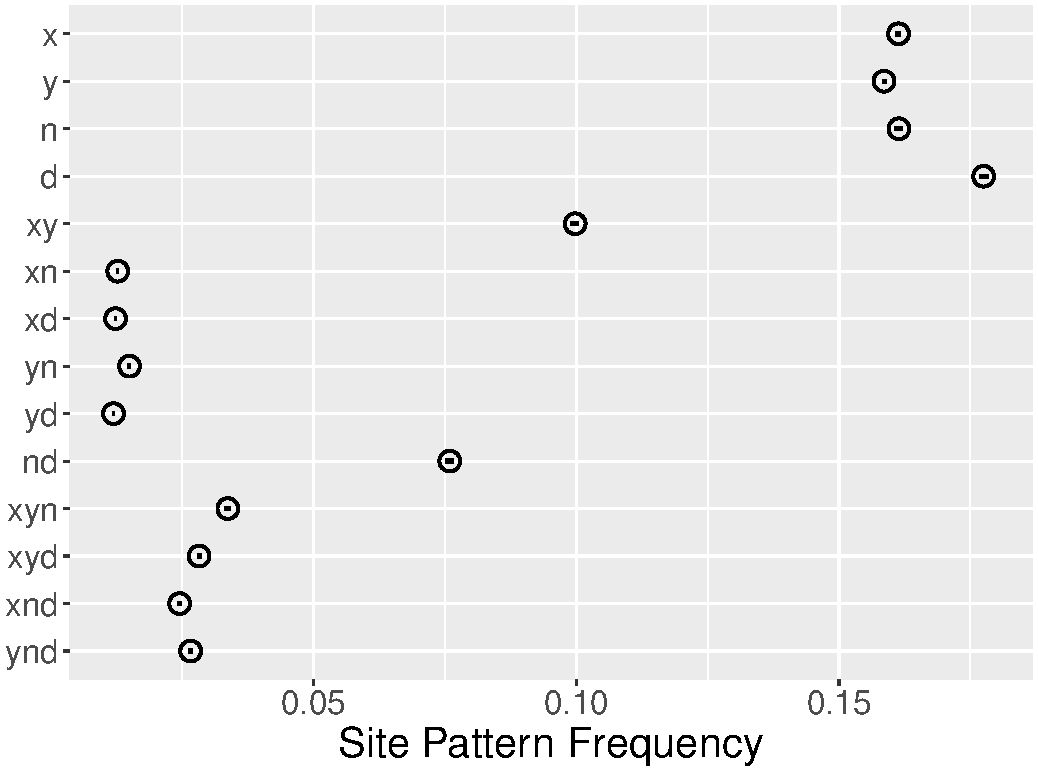
\includegraphics[width=\linewidth]{xynd-frq.pdf}
    \column{0.3\textwidth}
      \raggedleft

      $d$ most common singleton

      \bigskip

      \textit{xyn} most common tripleton

      \bigskip

      Signature of $S{\rightarrow}D$ gene flow (Pr{\"u}fer et al 2014).
  \end{columns}
\end{frame}

\begin{frame}
  \frametitle{What we learned, just by staring at the data}
  \begin{enumerate}
    \item Europeans and Africans are close relatives.
    \item So were Neanderthals and Denisovans.
    \item European-African separation more recent than
      Neanderthal-Denisovan.
    \item Neanderthals contributed genes to Europeans
    \item Superarchaics contributed genes to Denisovans.
  \end{enumerate}

  \bigskip
  
This analysis has been exploratory. Legofit extends these ideas to
estimate parameters and test hypotheses about history.
\end{frame}  

\end{document}


\begin{frame}
\frametitle{}
\end{frame}
